\documentclass[11pt,a4paper]{article}
\usepackage[hyperref]{acl2018}
\usepackage{times}
\usepackage{latexsym}

\usepackage[letterpaper]{geometry}
%\usepackage{amta2016}
\usepackage{url}
\usepackage{natbib}
\usepackage{layout}

\usepackage{algorithm}% http://ctan.org/pkg/algorithms
\usepackage{algpseudocode}% http://ctan.org/pkg/algorithmicx

\usepackage{graphicx}
\usepackage{amsmath}
\DeclareMathOperator*{\argmax}{argmax}

\newcommand{\confname}{AMTA 2016}
\newcommand{\website}{\protect\url{http://www.amtaweb.org/}}
\newcommand{\contactname}{research track co-chair Lane Schwartz}
\newcommand{\contactemail}{lanes@illinois.edu} 
\newcommand{\conffilename}{amta2016}
\newcommand{\downloadsite}{\protect\url{http://www.amtaweb.org/}}
\newcommand{\paperlength}{$12$ (twelve)}
\newcommand{\shortpaperlength}{$6$ (six)}

%% do not add any other page- or text-size instruction here

\parskip=0.00in

\begin{document}

% \mtsummitHeader{x}{x}{xxx-xxx}{2016}{45-character paper description goes here}{Author(s) initials and last name go here}
\title{\bf Faster Neural Machine Translation Inference}  

\author{\name{\bf Hieu Hoang} \hfill  \addr{hieu@hoang.co.uk}\\ 
        \addr{}
\AND
       \name{\bf Tomasz Dwojak} \hfill \addr{???}\\
        \addr{Adam Mickiewicz University}
\AND
       \name{\bf Kenneth Heafield} \hfill \addr{???}\\
       %\name{\bf Kenneth Heafield} \hfill \addr{kheafiel@inf.ed.ac.uk}\\
        \addr{University of Edinburgh, Scotland}
}

\maketitle
\pagestyle{empty}

\begin{abstract}

As neural machine translation (NMT) models have become the new state-of-the-art, the challenge is to make their deployment efficient and economical. We have identified two areas where typical NMT models differ significantly from other deep-learning models that impact on their inference speed. Firstly, NMT models usually contains a large number of output classes, corresponding to the output vocabulary. Secondly, rather than a single label, the output from machine translation models is a sequence of class labels that makes up the words or sub-words in the target sentence. Target sentence lengths are unpredictable, leading to inefficiencies during batch processing. We provide solutions for each of these issues which together increase batched inference speed by up to 57\% on modern GPUs without affecting model quality.

\end{abstract}

\section{Introduction}
\label{sec:Introduction}

We will examine two areas that are critical to fast NMT inference where the models differ significantly from other deep-learning models. We believe the optimizations of these models have been overlooked by the general deep-learning community.

Firstly, the number of classes in many deep-learning applications is small. However, the number of classes in NMT models is typically in the tens or hundreds of thousands, corresponding to the vocabulary size of the output language. For example, ~\cite{sennrich-haddow-birch:2016:P16-12} experimented with target vocabulary sizes of 60,000 and 90,000 sub-word units. This makes the output layer of NMT models very computationally expensive. Figure~\ref{fig:pie-time-europarl} shows the breakdown of amount of time during translation our NMT system; nearly 70\% of the time is involved in the output layer. We will look at optimizations which explicitly target the output layer.
\begin{figure}
\centering
\begin{tabular}{cc}
{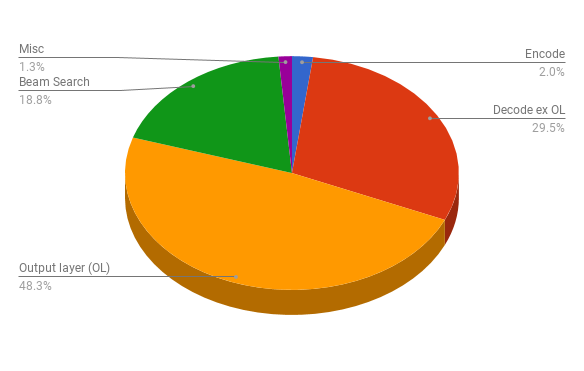
\includegraphics[scale=0.3]{pie-time-europarl.png}} 
\end{tabular}
\caption{Proportion of time spent during translation (Europarl test set)}
\label{fig:pie-time-europarl}
\end{figure} 

Secondly, the use of mini-batching is critical for fast model inference. However, mini-batching does not take into account variable sentence lengths which decrease the actual number of input or output sentences that are processed in parallel, negating the benefit of mini-batching. This can be partially reduced in the encoding with \emph{maxi-batching}, i.e. pre-sorting sentences by length before creating mini-batches with similar length source sentences. However, maxi-batching can introduce unacceptable delay in response for online applications as the input are not processed in the order they came. It is also not appropriate for applications where only the output lengths varies, for example, image captioning.

Even with sequence-to-sequence NMT models, target sentence lengths will still differ even for similar length inputs, compromising decoding performance. Figure~\ref{fig:batch-size} shows the actual batch size during decoding with a maximum batch size of 128; the batch was full in only 42\% of decoding iterations.

\begin{figure}
\centering
\begin{tabular}{cc}
{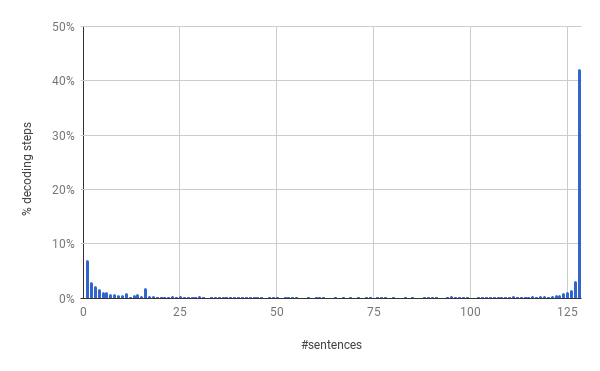
\includegraphics[scale=0.3]{batch-size.png}} 
\end{tabular}
\caption{Actual batch size during decoding (Europarl test set)}
\label{fig:batch-size}
\end{figure} 

We will propose an alternative batching algorithm to increase the actual batch size during decoding without the problems associated with mini-batching and maxi-batching.

We base our work on the sequence-to-sequence model of ~\cite{D14-1179}. We also choose to focus on the using NMT inference on GPUs. % rather than CPUs as pursued by ~\cite{DBLP:conf/emnlp/Devlin17}.

\section{Prior Work}

Deep-learning models has been successfully used on many machine learning task in recent years in areas as diverse as computer vision and natural language processing. This success have been followed by the rush to put these model into production. The computational resources required in order to run these models has been challenging but, fortunately, there has been a lot work to meet this challenge.

Hardware accelerators such as GPUs are very popular but other specialized hardware such as custom processors~\citep{DBLP:journals/corr/JouppiYPPABBBBB17} and FPGA~\citep{DBLP:journals/corr/LaceyTA16} have been used. Hardware-supported reduced precision is also an ideal way to speed up model inference~\citep{DBLP:journals/corr/abs-1710-03740}.

Simpler, faster models have been created that are as good, or almost as good, as more slower, more complex models~\citep{DBLP:journals/corr/BahdanauCB14}. Research have also gone into smaller, faster models that can approximate the original, slower, bigger model~\citep{DBLP:conf/emnlp/KimR16}. Some models have been justified as more suited for the parallel architecture of GPUs~\cite{DBLP:journals/corr/VaswaniSPUJGKP17}.

The speed of the softmax layer when used with large vocabularies have been looked at in~\citep{DBLP:journals/corr/GraveJCGJ16} but there have been many other attempts at faster softmax, for example~\cite{DBLP:journals/corr/abs-1301-3781}, ~\cite{Zoph-2016}.

There has been surprisingly little work on batching algorithms, considering its critical importance for efficient deep-learning training and inference. ~\cite{Neubig-autobatching} describe an novel batching algorithm, however, its aim is to alleviate the burden on developers in batching of new models, not faster batching.

Our paper follows most closely on from ~\cite{DBLP:conf/emnlp/Devlin17} which achieved faster NMT inference mainly by novel implementation of an existing model. However, we differ by focusing on GPU implementation, and the output layer and batching algorithm which were not touched on by the previous work.

\section{Proposal}
\label{sec:Proposal}

\subsection{Softmax and Beam Search Fusion}

The output layer of most deep learning models consist of the following steps
\begin{enumerate}
   \item \vspace{-2 mm} multiplication of the input with the weight vector $p = w x$
   \item \vspace{-2 mm} addition of a bias term to the resulting scores $p = p + b$
   \item \vspace{-2 mm} applying the activation function, most commonly softmax $ p_i = \exp(p_i) / \sum \exp(p_i) $
   \item \vspace{-2 mm} a beam search for the best (or n-best) output classes $\argmax_i p_i$
\end{enumerate}

In models with a small number of classes such as binary classification, the computational effort required is trivial and fast. However, this is not the case for large number of classes such as those found in NMT models.

We shall leave step 1 for future work and focus on the last three steps, the outline for which are shown in Algorithm~\ref{algo:original-softmax-beamsearch}. For brevity, we show the algorithm for 1-best, a beam search of the n-bests is a simple extension of this.

\begin{algorithm} 
\begin{algorithmic}

\Procedure{AddBias}{vector $p$, bias vector $b$}
\ForAll{$p_i$ in $p$}
  \State $p_i \gets p_i + b_i$
\EndFor 
\EndProcedure

\State

\Procedure{Softmax}{vector $p$}

\Comment{calculate max for softmax stability}
\State $max \gets - \infty$ 
\ForAll{$p_i$ in $p$}
  \If{$p_i > max$}
    \State $max \gets p_i$
  \EndIf
\EndFor

\Comment{calculate denominator} 
\State $sum \gets 0$ 
\ForAll{$p_i$ in $p$}
  \State $sum \gets sum + \exp(p_i - max)$
\EndFor

\Comment{calculate softmax}
\ForAll{$p_i$ in $p$}
  \State $p_i \gets \frac{\exp(p_i) - max}{sum} $
\EndFor 

\EndProcedure

\State

\Procedure{Find-Best}{softmax vector $p$}

\State $max \gets - \infty$ 
\ForAll{$p_i$ in $p$}
  \If{$p_i > max$}
    \State $max \gets p_i$
    \State $best \gets i$
  \EndIf
\EndFor 

\EndProcedure

\end{algorithmic}
\caption{Original softmax and beam Search Algorithm}
\label{algo:original-softmax-beamsearch}
\end{algorithm}


As can be seen, the operations iterate over the matrix p five times - once to add the bias, three times to calculate the softmax, and once to search for the best class. We shall use a popular method, kernel fusion~\citep{Guevara2009EnablingTP}, to optimize the output layer.

Secondly, we make use of the fact that softmax and $\exp$ are monotonic functions therefore we can move the search for the best class from FIND-BEST to SOFTMAX.

Thirdly, we are only interested in the probabilities of the best classes. Since these classes are known, we can avoid calculating softmax for all classes. The outline of the our function is shown in Algorithm~\ref{algo:Fused Kernel}.

\begin{algorithm}
\begin{algorithmic}
\Procedure{Fused-Kernel}{vector $p$, bias vector $b$}

\Comment{add bias, calculate $max$ \& $argmax$}

\State $max \gets - \infty$ 
\ForAll{$p_i$ in $p$}
  \If{$p_i + b_i > max$}
    \State $max \gets p_i + b_i$
    \State $best \gets i$
  \EndIf
\EndFor

\Comment{calculate denominator}

\State $sum \gets 0$ 
\ForAll{$p_i$ in $p$}
  \If{$p_i > max$}
    \State $sum \gets sum + \exp(p_i - max)$
  \EndIf
\EndFor

\Return $\frac{1}{sum}$, $best$ 

\EndProcedure
\end{algorithmic}

\caption{Fused softmax and beam search}
\label{algo:Fused Kernel}
\end{algorithm}

In fact, we are usually only interested in the best class during inference, not the probability. Therefore, we can skip the second iteration over $p$ in Algorithm~\ref{algo:Fused Kernel} and avoid computing the softmax altogether, Algorithm~\ref{algo:Argmax only}.

\begin{algorithm}
\begin{algorithmic}
\Procedure{Find-1-Best}{vector $p$, bias vector $b$}

\State $max \gets - \infty$ 
\ForAll{$p_i$ in $p$}
  \If{$p_i + b_i > max$}
    \State $max \gets p_i + b_i$
    \State $best \gets i$
  \EndIf
\EndFor

\Return $best$ 

\EndProcedure

\end{algorithmic}
\caption{Find 1 best only}
\label{algo:Argmax only}
\end{algorithm}

It has been shown ~\citep{koehn-knowles:2017:NMT} that using beam search to use the n-best number of classes, rather than just the best class, improves translation quality, up to a point. Unlike the 1-best case, however, the softmax calculation cannot be skipped as the denominator differs for each input.


\subsection{Top-up Batching}

The standard mini-batching algorithm is outlined in Algorithm~\ref{algo:Mini-batching}.

\begin{algorithm}
\begin{algorithmic}
\Procedure{Mini-Batching}{}
%\REQUIRE source sentence $s$, translation options
\While{more input} 
  \State Create batch $b$
  \State Encode($b$)
  \While{batch is not empty} 
    \State Decode($b$)
    \ForAll{sentence $s$ in $b$}
      \If{translation is complete}
        \State Remove $s$ from $b$
      \EndIf
    \EndFor
  \EndWhile
\EndWhile

\EndProcedure

\end{algorithmic}
\caption{Mini-batching}
\label{algo:Mini-batching}
\end{algorithm}

This algorithm encode the sentences for a batch, followed by decoding the batch. The decoding stop once all sentences in the batch are completed. This is a potential inefficiency as the number of remaining sentences may not be optimal.

We will focus on decoding as this is the more compute-intensive step, and issues with differing sentence sizes in encoding can partly be ameliorated by maxi-batching.

Our proposed top-up batching algorithm encode and decode asynchronously. The encoding step, Algorithm~\ref{algo:Encoding for top-up batching}, is similar to the main loop of the standard algorithm but the results are added to a queue to be consumed by the decoding step later.

\begin{algorithm}
\begin{algorithmic}

\Procedure{Encode}{}
\While{more input} 
  \State Create encoding batch $b$
  \State Encode($b$)
  \State Add $b$ to queue $q$
\EndWhile 

\EndProcedure

\end{algorithmic}
\caption{Encoding for top-up batching}
\label{algo:Encoding for top-up batching}
\end{algorithm}

Rather than decoding the same batch until all sentences in the batch are completed, the decoding step processing the same batch continuously. New sentences are added to the batch as old sentences completes, Algorithm~\ref{algo:Decoding for top-up batching}.

\begin{algorithm}
\begin{algorithmic}

\Procedure{Decode}{}

\State create batch $b$ from queue $q$
\While{$b$ is not empty}
  \State Decode($b$)
  \ForAll{sentence $s$ in $b$}
    \If{translation is complete}
      \State Replace $s$ with $s'$ from $q$
    \EndIf
  \EndFor
\EndWhile

\EndProcedure

\end{algorithmic}
\caption{Decoding for top-up batching}
\label{algo:Decoding for top-up batching}
\end{algorithm}


\section{Experimental Setup}
\label{sec:Experimental Setup}

We trained a sequence-to-sequence, encoder-decoder NMT system similar to that described in ~\cite{sennrich-haddow-birch:2016:P16-12}. This uses recurrent neural networks with gated recurrent units. The input and output vocabulary size were both set to 85,000 sub-words using byte-pair encoding (BPE) to adjust the vocabulary to the desired size. The hidden layer dimensions was set to 512. %We used the Marian toolkit to train our models.

For inference, we used and extend Amun~\citep{junczys2016neural}, the fastest open-source inference engine we are aware of for the model used in this paper. We used a beam size of 5, mini-batch of 128 sentences and maxi-batch 1280, unless otherwise stated.

The hardware used in all experiments was an Nvidia GTX 1060 GPU on a host containing 8 Intel hypercores running at 2.8Ghz, 16GB RAM and SSD hard drive.

Our training data consisted of the German-English parallel sentences from the Europarl corpus~\citep{Koehn:2005:MTS}. To test inference speed, we used two test sets with differing characteristics:
\begin{enumerate}
   \item \vspace{-2 mm} a subset of the Europarl training data, which contains mostly long sentences, and is, of course, in the same domain as the training data
   \item \vspace{-2 mm} a subset of the German-English data from the Open-Subtitles corpus, consisting of mostly short, out-of-domain sentences.
\end{enumerate}
Table~\ref{tab:corpora} gives further details of the test sets.

\begin{table}
\begin{center}
\small
\begin{tabular}{|l|r|r|} \hline
		  & Europarl		& OpenSubtitles \\ \hline
\# sentences  	  & 30,000 		& 50,000 \\
\# sub-words 	  & 787,908 		& 467,654 \\ 
Avg sub-words/sent & 26.3		& 9.4 \\
Std dev subwords/sent & 14.9		& 6.1 \\ \hline
\end{tabular}
\end{center}
\caption{Test sets}
\label{tab:corpora}
\end{table}


\section{Results}
\label{sec:Results}

\subsection{Softmax and Beam Search Fusion}

Fusing the last 3 steps led to a substantial reduction in the time taken, especially for beam size of 1 where the softmax probability does not actually have to calculated, Table~\ref{tab:fused-breakdown-europarl} and ~\ref{tab:fused-breakdown-opensubtitles}. This led to an overall increase in translation speed of up to 23\% for the Europarl test set, Figure~\ref{fig:beam-europarl}, and up to 41\% for the OpenSubtitles test set, Figure~\ref{fig:beam-opensubtitles}. 

The amount of time taken by the output layer dominates translation time for the OpenSubtitles test set, Figure~\ref{fig:pie-time-opensubtitles}, explaining the bigger overall translation speed with the fused kernel.

\begin{table}
\begin{center}
\small
\begin{tabular}{|l|r|r|} \hline
		& Baseline	& Fused \\ \hline
\multicolumn{3}{|c|}{\emph{Beam size 1}}	\\ \hline	
Multiplication 	& 25.62 	& 26.47 (+3.3\%) \\ \hline
Add bias 	& 4.98		&  \\ 
Softmax 	& 12.81		& 7.94 (-76.9\%)\\
Beam search	& 16.64		&  \\ \hline
\multicolumn{3}{|c|}{\emph{Beam size 5}}	\\ \hline	
Multiplication 	& 112.9 	& 115.04 (+1.9\%) \\ \hline
Add bias 	& 23.66		&  \\ 
Softmax 	& 56.61		& 67.58 (-56.5\%)\\
Beam search	& 75.12		&  \\ \hline
\end{tabular}
\end{center}
\caption{Time taken in sec (Europarl)}
\label{tab:fused-breakdown-europarl}
\end{table}

\begin{table}
\begin{center}
\small
\begin{tabular}{|l|r|r|} \hline
		& Baseline	& Fused \\ \hline
\multicolumn{3}{|c|}{\emph{Beam size 1}}	\\ \hline	
Multiplication 	& 21.47 	& 21.94 (+2.2\%) \\ \hline
Add bias 	& 33.59		&  \\ 
Softmax 	& 8.83		& 5.70 (-89.9\%)\\
Beam search	& 13.91		&  \\ \hline
\multicolumn{3}{|c|}{\emph{Beam size 5}}	\\ \hline	
Multiplication 	& 79.66 	& 80.01 (+4.4\%) \\ \hline
Add bias 	& 14.95		&  \\ 
Softmax 	& 36.86		& 42.91 (-64.4\%)\\
Beam search	& 68.80		&  \\ \hline
\end{tabular}
\end{center}
\caption{Time taken in sec (OpenSubtitles)}
\label{tab:fused-breakdown-opensubtitles}
\end{table}


\begin{figure}
\centering
\begin{tabular}{cc}
{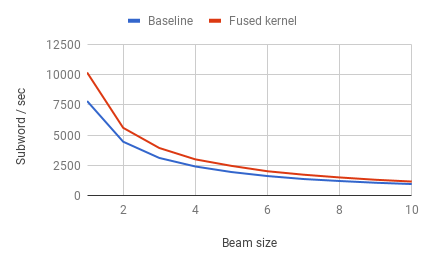
\includegraphics[scale=0.5]{beam-europarl.png}} 
\end{tabular}
\caption{Speed using the fused kernel (Europarl)}
\label{fig:beam-europarl}
\end{figure} 

\begin{figure}
\centering
\begin{tabular}{cc}
{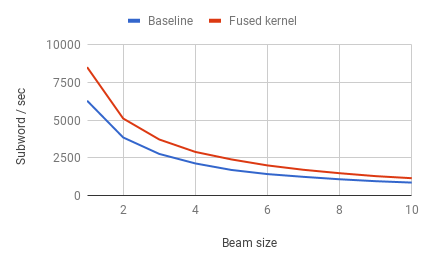
\includegraphics[scale=0.5]{beam-opensubtitles.png}} 
\end{tabular}
\caption{Speed using the fused kernel (OpenSubtitles)}
\label{fig:beam-opensubtitles}
\end{figure} 

\begin{figure}
\centering
\begin{tabular}{cc}
{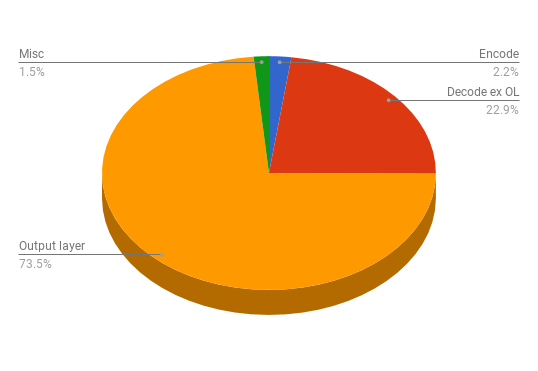
\includegraphics[scale=0.3]{pie-time-opensubtitles.png}} 
\end{tabular}
\caption{Proportion of time spent during translation (OpenSubtitles)}
\label{fig:pie-time-opensubtitles}
\end{figure} 


\subsection{Top-up Batching}

After some experimentation, we decided to top-up the decoding batch only when it is at least half empty, rather than whenever a sentence has completed.

The top-up batching and maxi-batching have similar goals of maximizing efficiency when translating batches of different lengths. Therefore, using both methods together gives limited gains, in fact, using top-up batching with maxi-batch slows of between 2\% to 18\% when translating the Europarl test set due to the overhead of using the algorithm, Figure~\ref{fig:topup-europarl}. When maxi-batching is inappropriate, using top-up batching alone matches the performance of maxi-batching, even being slightly faster when a small beam is used.

\begin{figure}
\centering
\begin{tabular}{cc}
{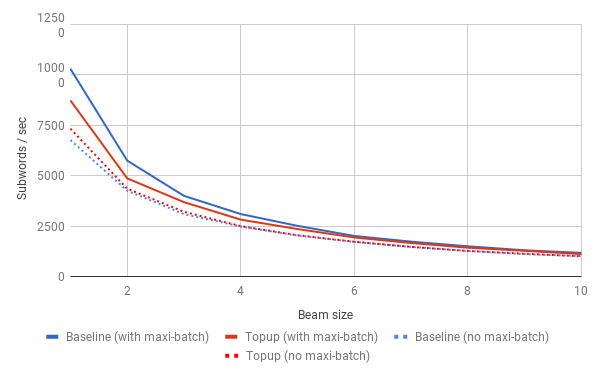
\includegraphics[scale=0.3]{topup-europarl.png}} 
\end{tabular}
\caption{Speed using top-up batching (Europarl)}
\label{fig:topup-europarl}
\end{figure} 

The results are better when translating the OpenSubtitles test set, Figure~\ref{fig:topup-opensubtitles}. The top-up batching does not harm performance when used with maxi-batching, even helping a little for small beams. However, top-up batching increases translation speed by up to 12\% when used alone.

\begin{figure}
\centering
\begin{tabular}{cc}
{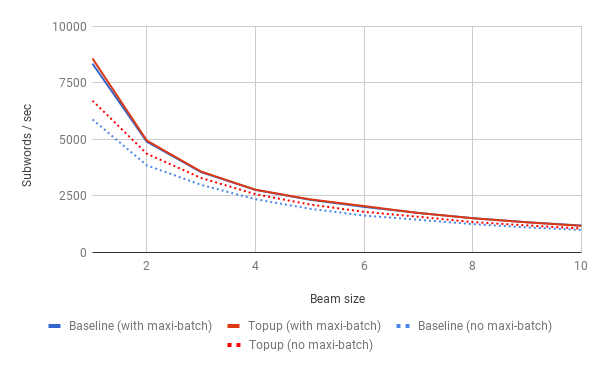
\includegraphics[scale=0.3]{topup-opensubtitles.png}} 
\end{tabular}
\caption{Speed using top-up batching (OpenSubtitles)}
\label{fig:topup-opensubtitles}
\end{figure} 

The gain from top-up batching is partially dependent on how much time the standard mini-batching algorithm spend decoding with a very small number of sentences as this is does not fully utilize the GPU cores. From Figure~\ref{fig:batch-size-small}, 20\% of the decoding iterations have less than 8 sentences remaining in the batch when translating the Europarl test test with maxi-batching. This figure is 50\% for the OpenSubtitles test set with no maxi-batching. The OpenSubtitles test set has a higher variance of sentence lengths relative to its average sentence length, which forces the mini-batch algorithm to continue decoding with a small number of sentences while the other sentences have already completed.

\begin{figure}
\centering
\begin{tabular}{cc}
{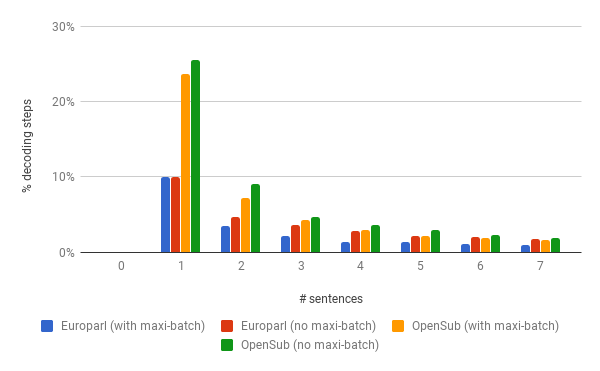
\includegraphics[scale=0.3]{batch-size-small.png}} 
\end{tabular}
\caption{Actual batch size during decoding}
\label{fig:batch-size-small}
\end{figure} 

\subsection{Cummulative Results}

Using both the fused kernel and top-up batching to translate led to a cummalative speed improvement of up to 57\% and 34\% for the OpenSubtitles and Europarl test set, respectively, when no maxi-batching is used, Figure~\ref{fig:cummulative-europarl} and Figure~\ref{fig:cummulative-opensubtitles}. With maxi-batching, the speed was up to 41\% and 21\%.

\begin{figure}
\centering
\begin{tabular}{cc}
{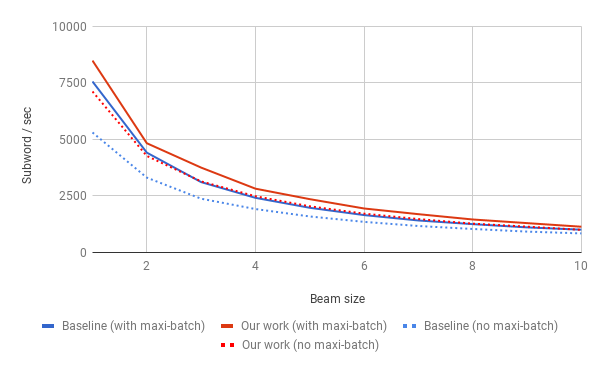
\includegraphics[scale=0.3]{cummulative-europarl.png}} 
\end{tabular}
\caption{Cummulative results (Europarl}
\label{fig:cummulative-europarl}
\end{figure} 

\begin{figure}
\centering
\begin{tabular}{cc}
{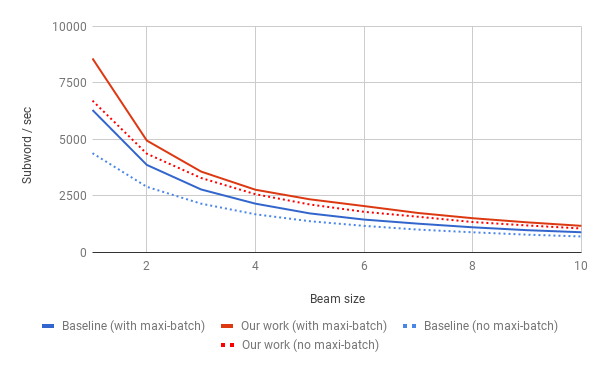
\includegraphics[scale=0.3]{cummulative-opensubtitles.png}} 
\end{tabular}
\caption{Cummulative results (OpenSubtitles}
\label{fig:cummulative-opensubtitles}
\end{figure} 

\section{Conclusion and Future Work}

We have presented two methods for faster deep-learning inference, targeted at neural machine translation. 

The first method focused on output layer of the neural network which accounts for a large part of the running time of the NMT model. By fusing the output layer with the beam search, we are able to increase translation speed by up to 41\%.

The second method replaces the mini-batching algorithm with one that avoids decoding with a small number of sentences, maximizing the parallel processing potential of GPUs. For certain scenarios, this increases translating  speed by up to 12\%.

For future work, we would like to apply our optimization for other NLP and deep-learning tasks. We are also interested in further optimization of the output layer in NMT, specifically the matrix multiplication which still takes up a significant proportion of the translation time.

%\section*{Acknowledgments}
%This work is sponsored by the Air Force Research Laboratory, prime contract FA8650-11-C-6160.  The views and conclusions contained in this document are those of the authors and should not be interpreted as representative of the official policies, either expressed or implied, of the Air Force Research Laboratory or the U.S. Government.

\bibliographystyle{apalike}
\bibliography{amta2016,mt,more}


\end{document}
\grid
